

\documentclass[a4paper,12pt]{article}
%%%%%%%%%%%%%%%%%%%%%%%%%%%%%%%%%%%%%%%%%%%%%%%%%%%%%%%%%%%%%%%%%%%%%%%%%%%%%%%%%%%%%%%%%%%%%%%%%%%%%%%%%%%%%%%%%%%%%%%%%%%%%%%%%%%%%%%%%%%%%%%%%%%%%%%%%%%%%%%%%%%%%%%%%%%%%%%%%%%%%%%%%%%%%%%%%%%%%%%%%%%%%%%%%%%%%%%%%%%%%%%%%%%%%%%%%%%%%%%%%%%%%%%%%%%%

\voffset=-1.0cm
\oddsidemargin=0.0cm
\textwidth = 490pt
\usepackage{eurosym}
\usepackage{vmargin}
\usepackage{amsmath}
\usepackage{graphics}
\usepackage{epsfig}
\usepackage{subfigure}
\usepackage{fancyhdr}
%\usepackage{listings}
\usepackage{framed}
\usepackage{graphicx}
\usepackage{amsmath}
\usepackage{enumerate}
\usepackage{chngpage}
\usepackage{multicol}
%\usepackage{bigints}


\setcounter{MaxMatrixCols}{10}
%TCIDATA{OutputFilter=LATEX.DLL}
%TCIDATA{Version=5.00.0.2570}
%TCIDATA{<META NAME="SaveForMode" CONTENT="1">}
%TCIDATA{LastRevised=Wednesday, February 23, 2011 13:24:34}
%TCIDATA{<META NAME="GraphicsSave" CONTENT="32">}
%TCIDATA{Language=American English}

%\pagestyle{fancy}
%\setmarginsrb{20mm}{0mm}{20mm}{25mm}{12mm}{11mm}{0mm}{11mm}
%\lhead{MA4413} \rhead{Mr. Kevin O'Brien}
%\chead{Statistics For Computing}
%\input{tcilatex}

\begin{document}

%====================================================%
\begin{center}
	
\includegraphics[scale=0.65]{images/shieldtransparent2}
\end{center}

\begin{center}
	\vspace{1cm}
	\large \bf {FACULTY OF SCIENCE AND ENGINEERING} \\[0.5cm]
	\normalsize DEPARTMENT OF MATHEMATICS AND STATISTICS \\[1.25cm]
	\large \bf {EXAMINATION PAPER 2016} \\[1.5cm]
\end{center}

\begin{tabular}{ll}
	MODULE CODE: MA4505 & SEMESTER: Autumn 2016 \\[1cm]
	MODULE TITLE: Applied Statistics  & DURATION OF EXAM: 2.5 hours \\
\phantom{MODULE TITLE:} for Administration 1 & \phantom{ DURATION OF EXAM: 2.5 hours} \\[1cm]
	LECTURER: Mr. Kevin O'Brien & GRADING SCHEME: 100 marks \\
	& \phantom{GRADING S} \footnotesize {(60\% of Module Grade)} \\[0.8cm]
	EXTERNAL EXAMINER: Prof. A. Marshall & \\
\end{tabular}
\bigskip
\begin{center}
	{\bf INSTRUCTIONS TO CANDIDATES}
\end{center}

{\noindent \\ Scientific calculators approved by the University of Limerick can be used. \\
	Formula sheet and statistical tables are provided at the end of the exam paper.\\
	Students must attempt any 4 questions from 5.}
\newpage
\section*{Question 1. (25 marks) Descriptive Statistics}
\subsubsection*{Part A - Graphical Methods (15 Marks)} %28 MARKS
The exam results for a class of 60 students are tabulated below.
\begin{table}[ht]
	\centering
	\begin{tabular}{|rrrrrrrrrr|}
		\hline
	
	  19 &  25 &  30 &  35 &  35 &  36 &  36 &  37 &  37 &  38 \\ 
	  38 &  38 &  39 &  39 &  40 &  43 &  43 &  43 &  44 &  45 \\ 
		 46 &  47 &  47 &  47 &  47 &  47 &  48 &  48 &  49 &  49 \\ 
	  50 &  51 &  52 &  53 &  53 &  53 &  54 &  56 &  57 &  57 \\ 
		  59 &  60 &  60 &  60 &  61 &  62 &  63 &  63 &  64 &  64 \\ 
		  65 &  66 &  69 &  72 &  78 &  85 &  88 &  89 &  93 &  99 \\ 
		\hline
	\end{tabular}
\end{table}
\vspace{-0.5cm}
\begin{enumerate}[(i)]
	\item (3 Marks) Summarize the data in the above table using a relative frequency table, a cumulative frequency table, and a cumulative relative frequency table. Use 9 class intervals, with 11 as the lower limit of the first interval.
	\item (6 Marks) Draw a histogram for the above data. Comment on the shape of the histogram. Based on the shape of the histogram, what is the best measure of centrality and variability?
	\item (6 Marks) Construct a box plot for the above data. Clearly demonstrate how all of the necessary values were computed.
\end{enumerate}

\vspace{0.25cm}
\subsubsection*{Part B - Summary Statistics (5 Marks)} %10 MARKS
Data on the durations (measured in months) were collected for a random sample of product development projects. The durations for these development projects are as follows:

\begin{table}[ht]
	\centering
	\begin{tabular}{|rrrrrrrr|}
		\hline
		
		16 &  20 &  14 &  29 &  30 &  22 &  21 &  28 \\ 
		\hline
	\end{tabular}
\end{table}	
\vspace{-0.5cm}


\begin{enumerate}[(i)]
	\item (1 Mark) Calculate the mean project duration.
	\item (1 Mark) Calculate the median project duration.
	\item (2 Marks) Calculate the variance of the project durations.
	\item (1 Mark) Calculate the standard deviation of the project durations.
\end{enumerate}


%\subsection*{Part A - Boxplots (6 Marks)}
%Construct a pair of box plots for the data in the below. Construct one box plot for the data related to Material A, the other for Material B. Comment on the features of the box plots and what conclusions, if any, you can derive from the two box plots.
%\begin{center}
%	\begin{tabular}{|c|c|l|}
%		\hline
%		Material & Sample size & Bonding Strength (Newton Metres) \\ \hline
%		
%		A (80\% pure) & 12 & 2.0 2.1 2.1 2.1 2.2 2.3 2.3 2.3 2.4 2.4 2.5 2.6
%		\\ \hline
%		
%		B (60\% pure) & 10 & 1.9 1.9 2.0 2.1 2.1 2.2 2.2 2.5 2.7 2.8 \\ \hline
%	\end{tabular} 
%\end{center}
%\medskip
%\textit{
%	\noindent Marking Scheme:
%	\begin{itemize}
%		\item 4 Marks for showing the relevant calculations,
%		\item 1 Mark for drawing the boxplots to a satisfactory standard.
%		\item 1 Mark for a well-explained conclusion,
%	\end{itemize}
%}

\newpage

\subsection*{Part C - Dixon Q Test (5 Marks)}


Use the Dixon Q Test to determine if the lowest value is an outlier. You may assume a significance level of 5\%.
	\[ 131, 136, 101, 126, 123, 120, 132, 137\]
\begin{itemize}
	\item[(i)](1 Mark)	State the null and alternative hypotheses for this test.
	\item[(ii)](2 Marks) Compute the test statistic
	\item[(iii)](1 Mark) State the appropriate critical value.
	\item[(iv)](1 Mark) What is your conclusion to this procedure.
\end{itemize}	


\section*{Question 2. (25 marks) Probability Distributions }

\subsection*{Part A - Normal Distribution (10 Marks)}

\smallskip	
\noindent Assume that the diameter of a critical component is normally distributed with a mean of 500mm and a standard deviation of 12.5mm. You are required  to estimate the approximate probability of the following measurements occurring on an individual component.
\begin{itemize}
	\item[(i)](2 Mark) Greater than 517mm.
	\item[(ii)](3 Marks) Less than 495mm.
	\item [(iii)](2 Marks) Between 495mm and 513mm.
		\item[(iv)] (3 Marks) The production manager reports that more than 99\% of the output is between 475mm and 525mm. Do you agree with this statement? Justify your answer with the appropriate calculations.
\end{itemize}
\medskip
\noindent Use statistical tables to determine the probabilities for the above exercises. You are required to show all of your workings.

%
%
%\subsection*{Part B - Normal Distribution (10 Marks)} % Normal %6 MARKS
%Assume that the diameter of a critical component is normally distributed with a Mean of 100mm and a Standard Deviation of 5mm. You are required  to estimate the approximate probability of the following measurements occurring on an individual component.
%\begin{itemize}
%	\item[(i)](1 Mark)	Greater than 104.1mm
%	\item[(ii)](2 Marks) Less than 95.2 mm
%	\item [(iii)](2 Marks) Between 94.2 and 103 mm
%\end{itemize}


\subsection*{Part B - Probability (10 Marks)} % Normal %6 MARKS
A new test has been developed to diagnose a particular disease. If a person has the disease, the test has a 95\% chance of identifying them as having the disease. 
If a person does not have the disease, the test has a 1\% chance of identifying them as having the disease. Suppose that 5\% of the population have this disease. Suppose we select a person at random from the population.


\begin{enumerate}[(i)]
	\item (4 Marks) What is the probability that the test will identify them as having the disease?
	
	\item (3 Marks) What is the probability that the person has the disease given that the test identifies them as having the disease?
	\item (3 Marks) What is the probability that the person has the disease given that the test identifies them as \textbf{not} having the disease?
\end{enumerate}


%=================================================================%

\subsection*{Part C - Testing Distributional Assumptions (8 Marks)}
Consider the results of a statistical analysis carried out on sample data for the random variable $Y$. These results are presented as output from a statistical computer program.

\begin{itemize}
	\item[(i)] (1 Mark) What sort of statistical analysis are we carrying out? 
	\item[(ii)] (1 Mark) What is the relevance of this analysis as part of an overall statistical study.
	\item[(ii)] (2 Mark) Interpret the output of the Anderson-Darling Test. (\textit{Remark: Use a 5\% significance level. This test is a one-tailed procedure.})
	\item[(iv)] (1 Mark) What is the conclusion of this analysis for the variable $X$? Justify your answer with reference to 3 separate indications. 
	
\end{itemize}

\noindent (\textit{Computer results continue on the next page.})
%\bigskip
%\textit{\textbf{Important:} Question 3 comprises a third part: Part C. This part is presented in subsequent pages.}

\begin{figure}[h!]
	\centering
	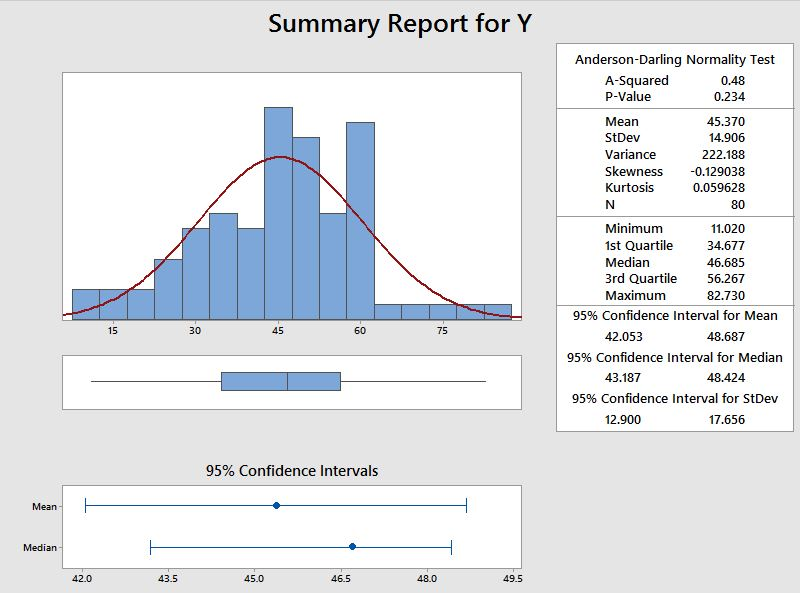
\includegraphics[width=0.99\linewidth]{images/NormalityTesting3}
\end{figure}
\begin{figure}[h!]
	\centering
	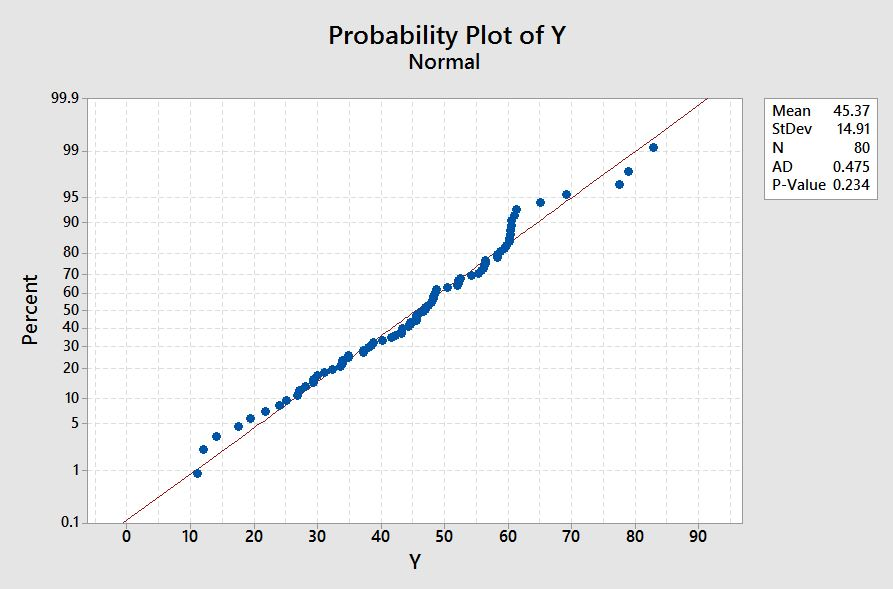
\includegraphics[width=0.99\linewidth]{images/NormalityTesting4}
\end{figure}

\newpage

%===============================================%




\newpage
\section*{Question 3. (25 marks) Single Sample Inference Procedures }
\subsubsection*{Part A - Single Sample Inference Procedures (15 Marks)}
Mean blood iron concentration for children with adequate nutrition is taken to be 110mg/dl. \\ \smallskip

\noindent 25 randomly selected children from a disadvantaged urban area were given blood tests. The mean concentration of iron from this sample was 98 mg/dl with a standard deviation of 25.5 mg/dl.
\begin{itemize}
	\item[(i)] (4 Marks) Calculate a 95\% confidence interval for the mean concentration of iron for children in this area. 
	\item[(ii)](2 Marks) Interpret this confidence interval.  Do these results provide evidence that children in this area suffer from iron deficiency? 
\end{itemize}
\medskip
Test this hypothesis using a 5\% level of significance. 

\begin{itemize}
	\item[(iii)](3 Marks) Formally state your null and alternative hypotheses.
	\item[(iv)](4 Marks) Compute the test statistic.
	\item[(v)](2 Marks) Discuss your conclusion to this test, supporting your statement with reference to appropriate values.
\end{itemize}





\subsubsection*{Part B  - Single Sample Proportion (10 Marks)}
%% Change the Numbers
An environmental group states that fewer than 60\% of industrial plants comply with air pollution standards. An independent researcher takes a sample of 400 plants and finds that 270 are complying with air pollution standards. 
\begin{itemize}
	\item[(i)] (5 Marks) Carry out a hypothesis test to investigate the claim made by the environmental group. Clearly state your null and alternative hypotheses and your conclusion.
	\item[(i)](3 Marks) Compute the 95\% confidence interval.
	%	\item[(ii)](3 Marks) Compute the Test Statistic.
	\item[(ii)](2 Marks) By interpreting this confidence interval, state your conclusion about the environmental group's claim? Explain how you made this decision.
\end{itemize}

%\subsubsection*{Part A} %4 Marks
%\begin{itemize}
%	\item[i.](2 Marks) In the context of hypothesis testing, explain what a p-value is, and how it is used. Support your answer with a simple example.
%	\item[ii.](2 Marks) What is meant by Type I error and Type II error?
%\end{itemize}
%\subsubsection*{Part B - Single Sample Proportion (10 Marks)} %3 Marks
%A well-known polling company estimates that $66\%$ of Irish voters support a new constitutional amendment. 700 people were randomly surveyed and asked about their voting preferences. 490 of the 700 people responded positively to the amendment. You are required to:
%
%\begin{itemize}
%	\item [i.](1 Mark) Obtain a point estimate of the proportion of people supporting the constitutional amendment.
%	\item [ii.](2 Marks) Construct a 95\% confidence interval for the proportion of people in favour of the constitutional amendment.
%\end{itemize}

%\subsubsection*{Part C - Test for Equal Variance (5 Marks)} %4 Marks
%The standard deviations of data sets \texttt{X} and \texttt{Y} are 12 and 10 respectively.
%
%\begin{center}
%\begin{tabular}{|c|c|c|} \hline
%	Sample &Sample Mean ($\bar{x}$)& Sample Std. Deviation ($s$)\\ \hline
%	X & 100.126 & 3.256 \\ \hline
%	Y & 104.422 & 6.638 \\ \hline
%\end{tabular}
%\end{center}
%
%
%
% An inference procedure was carried out to assess whether or not \texttt{X} and \texttt{Y} can be assumed to have equal variance.
%\begin{itemize}
%	\item[i.](1 Mark) Formally state the null and alternative hypothesis.
%	\item[ii.](1 Mark) The Test Statistic has been omitted from the computer code output. Compute the value of the Test Statistic.
%	\item[iii.](2 Marks) What is your conclusion for this procedure? Justify your answer.
%	%\item[iv.] (1 Marks) Explain how a conclusion for this procedure can be based on the $95\%$ confidence interval.
%\end{itemize}
%
%%---- R code for Variance Test ----%
%%---- Dummy Code Included                   ----%
%\begin{framed}
%	\begin{verbatim}
%> var.test(X,Y)
%
%F test to compare two variances
%
%data:  X and Y
%
%F = ........., num df = 11, denom df = 14, p-value = 0.02272
%alternative hypothesis: true ratio of variances is not equal to 1
%95 percent confidence interval:
%0.07777832 0.80843870
%sample estimates:
%ratio of variances 
%.........
%
%
%
%	\end{verbatim}
%\end{framed}
%======================================================================%


\section*{Question 4. (25 marks) Two Sample Inference Procedures }

%\subsection*{Part A (10 Marks)}
%
%\begin{itemize}
%	\item In a survey of perceived health risks in Dublin, each member of a random
%	sample of 200 people was asked the question "\textit{When buying food, do you check the
%		pack for artificial additives?}". 
%	
%	\item The researchers wanted to discover whether females or
%	males were more likely to check for artificial additives when buying food.
%\end{itemize}
%
%
%\begin{center}
%	\begin{tabular}{|c|c|c|}
%		\hline 
%		&  Yes & No \\ 
%		
%		\hline 
%		Female	& 60 & 60 \\ 
%		\hline 
%		Male	& 32 & 48  \\ 
%		\hline 
%	\end{tabular} 
%\end{center}
%Using a 5\% significance level, test for a difference between the percentages of males and females responding ``Yes" to the question about checking for artificial additives.
%
%	
%\begin{itemize}
%	\item[(i)](3 Marks) Clearly state your null and alternative hypotheses.
%	\item[(ii)](4 Marks) Compute the Test Statistic.
%	\item[(iii)](3 Marks) Discuss your conclusion to this test, supporting your statement with reference to appropriate values.
%\end{itemize}
%	





\subsection*{Part A - Two Sample Test for Means (10 Marks)}
An exercise physiologist wants to determine if several short bouts of exercise provide the same benefit for cardiovascular fitness as one long bout of exercise. \\ \smallskip

\noindent 50 volunteers are randomly assigned to group 1 and do standardised aerobic exercise on a stationary bicycle for 30 minutes once a day, 5 days a week. 40 volunteers are randomly assigned to group 2 and do the same exercise for 10 minutes, 3 times a day, 5 days a week. Cardiovascular fitness was measured by VO2 max (maximum oxygen consumption while exercising). 

\begin{description}
	\item[Group 1] The mean change in VO2 after 12 weeks of exercise was 2.1 for group 1 with a standard deviation of 1.7.
	\item[Group 2] The mean change in VO2 after 12 weeks of exercise was 0.7 for group 2 with a standard deviation of 1. 
\end{description}

\noindent Test the hypothesis that there is no significant difference between two groups are the same.
	
\begin{itemize}
	\item[(i)](3 Marks) Formally state your null and alternative hypotheses.
	\item[(ii)](4 Marks) Compute the test statistic.
	\item[(iii)](3 Marks) Discuss your conclusion to this test, supporting your statement with reference to appropriate values.
\end{itemize}
\subsection*{Part B - Paired T Test (15 Marks)} %9 Marks
A microbiologist measures the total growth in 24 hours of two strains of a germ culture  in the same petri dish. Nine identical specimens are prepared. The growth rate for the eight samples for each strain are tabulated below:

\begin{center}
	\begin{tabular}{|c|c|c|} \hline 
		Specimen &	Strain 1	&	Strain 2	\\ \hline \hline
		1 & 212 & 224 \\ \hline
		2 & 234 & 231 \\ \hline
		3 & 214 & 209 \\ \hline
		4 & 236 & 243 \\ \hline
		5 & 221 & 231 \\ \hline 
		6 & 212 & 216 \\ \hline
		7 & 202 & 213 \\ \hline 
		8 & 210 & 216 \\ \hline
		9 & 248 & 242 \\ \hline
	\end{tabular} 
\end{center}
\noindent At a significance level of 5\%, is there sufficient evidence to state that there is any difference in growth rates between the two strains.


% State your hypotheses clearly. What is the significance level of this test?
\bigskip

\begin{itemize}
	\item[(i)](3 Marks) Formally state the null and alternative hypotheses.
	\item[(ii)] (3 Marks) Compute the mean and standard deviation of the case-wise differences.
	\item[(iii)](3 Marks) Compute the test statistic.
	\item[(iv)](3 Marks) State the appropriate critical value for this hypothesis test.
	\item[(v)](3 Marks) Discuss your conclusion to this test, supporting your statement with reference to appropriate values.
\end{itemize}

%        1-sample proportions test with continuity correction
%
% data:  482 out of 800, null probability 0.57
% X-squared = 3.3162, df = 1, p-value = 0.0686
% alternative hypothesis: true p is not equal to 0.57
% 95 percent confidence interval:
% 0.5675450 0.6364573
% sample estimates:
%     p
% 0.6025
%======================================================================%
\newpage

\section*{Question 5. (25 marks) Linear Regression Models and Chi Square Tests }
\subsection*{Part A - Chi Square Tests (10 Marks)}
A market research survey was carried out to assess preferences for three brands of chocolate bar, A, B, and C. 
The study group was categorised by maturity level to determine any difference in preferences. The purpose of this study is to assess differing preferences for brands across age groups.


{
\begin{center}
\begin{tabular}{|c||c|c|c||c|} \hline
	&	Brand A	&	Brand B	&	Brand C	&	Total	\\ \hline		\hline
	Children	&	65	&	55	&	30	&	150	\\ \hline	
	Teenages	&	35	&	75	&	40	&	150	\\ \hline	
	Adults	&	50	&	20	&	30	&	100	\\ \hline	\hline
	&	150	&	150	&	100	&	400	\\ \hline	 
\end{tabular} 
\end{center}
}
\begin{enumerate}[(i)]
	\item (1 Mark) Formally state the null and alternative hypotheses.
	\item (2 Marks) Compute each of the cell values expected under the null hypothesis. 
	\item (4 Marks) Compute the test statistic.
	\item (1 Mark) State the appropriate critical value for this hypothesis test.
	\item (2 Marks) Discuss your conclusion to this test, supporting your statement with reference to appropriate values.
\end{enumerate}




\subsection*{Part B - Linear Regression (15 Marks)}

An experiment was conducted to study the relationship between baking temperature x (in units of 10 degrees Farenheit) and yield y (as percentage) of popular cake mix. Fourteen observations were made giving the following results.

%Temp 10 10.5 11 11.5 12 15 17 19 20 21 23 25 27 30

%Yield 21.2 19.9 22.5 23.7 25 30.3 36.1 38.6 41.5 42.7 45 50 53.9 62.1



\begin{center}
\begin{tabular}{|c||c|c|c|c|c|c|c|}
\hline
Specimen & 1 & 2 & 3 & 4 & 5 & 6 & 7 \\ \hline
\hline
Temp &  10.00 & 10.50 & 11.00 & 11.50 & 12.00 & 15.00 & 17.00 \\ \hline 
Yield &  29.830&  26.370 & 30.325 &36.100 &33.410 &36.335 & 40.655 \\ \hline 
\hline\hline
Specimen & 8 & 9 & 10 & 11 & 12 & 13 & 14 \\  \hline
Temp &  19.00 & 20.00 & 21.00 & 23.00 & 25.00 & 27.00 & 30.00 \\ \hline
Yield &  39.475& 44.555&  42.015 & 47.795 & 45.560&  51.045 & 47.900 \\ \hline 
\hline
\end{tabular}
\end{center}

\begin{multicols}{3}
\begin{itemize}
	\item $S_{XX} = 570.5$
	\item $S_{YY} =  751.1525$
	\item $S_{XY} = 613.27$
	\item $\bar{X} = 18$
	\item $\bar{Y} = 39.383$
\end{itemize}
\end{multicols}
\medskip
\textit{(This question is continued on the next page.)}
\newpage

\begin{figure}
	\centering
	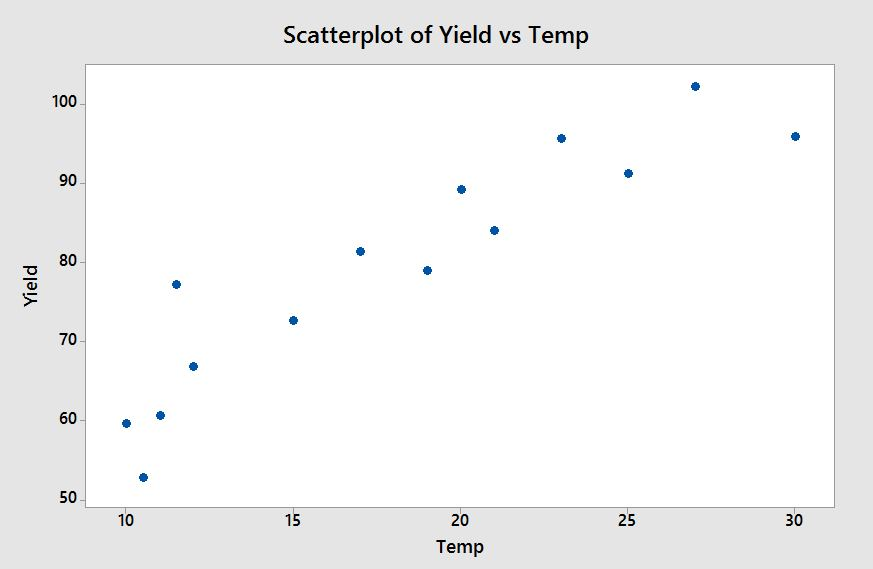
\includegraphics[width=0.99\linewidth]{images/MA4505RegressionPlot}
\end{figure}
\medskip
\begin{enumerate}[(i)]

	\item (2 Marks) Using the scatter plot, describe the relationship between the yield (Y) and the baking temperature (X).





		\item (4 Marks) Calculate the correlation coefficient. Interpret your answer.
		\item (6 Marks) Calculate the equation of the least squares regression line and interpret the value of the slope.
		\item (3 Marks) Using this regression model, estimate the yield when the baking temperature is 16 degrees.
%		\item (2 Marks) How much of the variation in yield is explained by fitting the regression line?
\end{enumerate}



%
%\begin{figure}
%\centering
%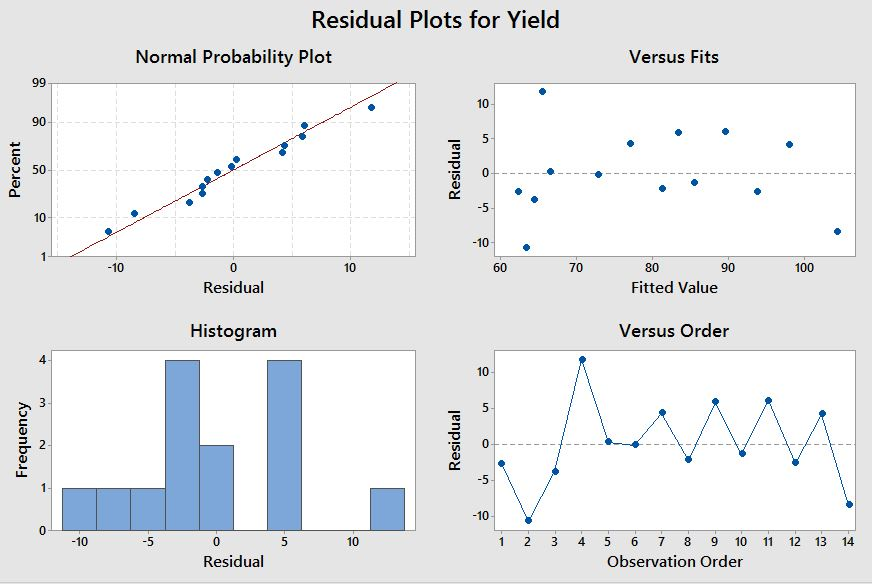
\includegraphics[width=0.99\linewidth]{images/MA4505RegressionResiduals}
%\caption{}
%\label{fig:MA4505RegressionResiduals}
%\end{figure}

%======================================================================%
\newpage





\section*{Formulae}
%-------------------------------------------------%
\subsection*{Descriptive Statistics}
\begin{itemize}
	\item Sample Variance
	\begin{equation*}
	s^2 = \frac{\sum (x-\bar{x})^2}{n-1}
	\end{equation*}
\end{itemize}
%-------------------------------------------------%
\subsection*{Probability}
\begin{itemize}
	
	\item Conditional probability:
	\begin{equation*}
	P(B|A)=\frac{P\left( A\text{ and }B\right) }{P\left( A\right) }.
	\end{equation*}
	
	
	\item Bayes' Theorem:
	\begin{equation*}
	P(B|A)=\frac{P\left(A|B\right) \times P(B) }{P\left( A\right) }.
	\end{equation*}
	
	
	
	
	%	
	%	\item Binomial probability distribution:
	%	\begin{equation*}
	%		P(X = k) = ^{n}C_{k} \times p^{k} \times \left( 1-p\right) ^{n-k}\qquad \left( \text{where  }
	%		^{n}C_{k} =\frac{n!}{k!\left(n-k\right) !}. \right)
	%	\end{equation*}
	%	
	%	\item Poisson probability distribution:
	%	\begin{equation*}
	%		P(X = k) =\frac{m^{k}\mathrm{e}^{-m}}{k!}.
	%	\end{equation*}
	%	
	%	\item Exponential probability distribution:
	%	\begin{equation*}
	%		P(X \leq k) = \begin{cases}
	%			1-e^{- k/\mu}, & k \ge 0, \\
	%			0, & k < 0.
	%		\end{cases}\qquad \left( \text{where  }
	%		\mu = {1\over \lambda}\right)
	%	\end{equation*}
\end{itemize}

\subsection*{Confidence Intervals}
{\bf One sample}
\begin{eqnarray*} S.E.(\bar{X})&=&\frac{\sigma}{\sqrt{n}}.\\\\
	S.E.(\hat{P})&=&\sqrt{\frac{\hat{p}\times(1-\hat{p})}{n}}.\\
\end{eqnarray*}
{\bf Two samples}
\begin{eqnarray*}
	S.E.(\bar{X}_1-\bar{X}_2)&=&\sqrt{\frac{\sigma^2_1}{n_1}+\frac{\sigma_2^2}{n_2}}.\\\\
	S.E.(\hat{P_1}-\hat{P_2})&=&\sqrt{\frac{\hat{p}_1\times(1-\hat{p}_1)}{n_1}+\frac{\hat{p}_2\times(100-\hat{p}_2)}{n_2}}.\\\\
\end{eqnarray*}
\subsection*{Hypothesis tests}
{\bf One sample}
\begin{eqnarray*}
	S.E.(\bar{X})&=&\frac{\sigma}{\sqrt{n}}.\\\\
	S.E.(p)&=&\sqrt{\frac{p \times(1-p)}{n}}
\end{eqnarray*}
{\bf Two large independent samples}
\begin{eqnarray*}
	S.E.(\bar{X}_1-\bar{X}_2)&=&\sqrt{\frac{\sigma^2_1}{n_1}+\frac{\sigma_2^2}{n_2}}.\\\\
	S.E.(\hat{P_1}-\hat{P_2})&=&\sqrt{\left(\bar{p}\times(1-\bar{p})\right)\left(\frac{1}{n_1}+\frac{1}{n_2}\right)}.\\
\end{eqnarray*}
{\bf Two small independent samples}
\begin{eqnarray*}
	S.E.(\bar{X}_1-\bar{X}_2)&=&\sqrt{s_p^2\left(\frac{1}{n_1}+\frac{1}{n_2}\right)}.\\\\
	s_p^2&=&\frac{s_1^2(n_1-1)+s_2^2(n_2-1)}{n_1+n_2-2}.\\
\end{eqnarray*}
{\bf Paired sample}
\begin{eqnarray*}
	S.E.(\bar{d})&=&\frac{s_d}{\sqrt{n}}.\\\\
\end{eqnarray*}
{\bf Standard Deviation of case-wise differences (computational formula)}
\begin{eqnarray*}
	s_d = \sqrt{ {\sum d_i^2 - n\bar{d}^2 \over n-1}}.\\\\
\end{eqnarray*}
\subsection*{Chi Square Tests of Independence}
\[\chi^2_{TS} =  \sum \frac{(n_{ij} - e_{ij})^2}{e_{ij}}\]
\subsection*{Regression Estimates}

\begin{eqnarray*}
	S_{XY} &=&
	\sum x_iy_i - \frac{\sum x_i\sum y_i}{n}\\
	S_{XX} &=&
	\sum x_i^2 - \frac{(\sum x_i)^2}{n}\\
	S_{YY} &=&
	\sum y_i^2 - \frac{(\sum y_i)^2}{n}\\
\end{eqnarray*}
{\bf Pearson's correlation coefficient}

\begin{eqnarray*}
	r = \frac{S_{XY}}{\sqrt{S_{XX} \times S_{YY}}}
\end{eqnarray*}

{\bf Slope Estimate}
\begin{eqnarray*}
	b_1 = \frac{S_{XY}}{S_{XX}}
\end{eqnarray*}
{\bf Intercept Estimate}
\begin{eqnarray*}
	b_0 = \bar{y} -b_1\bar{x}
\end{eqnarray*}

%{\bf Standard error of the Slope}
%\begin{eqnarray*}
%	S.E.(b1) = \sqrt{\frac{s^2}{S_{XX}}}
%\end{eqnarray*}
%
%where $s^2 = \frac{SSE}{n-2}$
%and SSE $= S_{YY} - b_1S_{XY}$

\subsection*{Critical Values for Dixon Q Test}
{
	\Large
	\begin{center}
		\begin{tabular}{|c|c|c|c|}
			\hline  n  & $\alpha=0.10$  & $\alpha=0.05$  & $\alpha=0.01$  \\ \hline
			3  & 0.941 & 0.970 & 0.994 \\ \hline
			4  & 0.765 & 0.829 & 0.926 \\ \hline
			5  & 0.642 & 0.710 & 0.821 \\ \hline
			6  & 0.560 & 0.625 & 0.740  \\ \hline
			7  & 0.507 & 0.568 & 0.680  \\ \hline
			8  & 0.468 & 0.526 & 0.634 \\ \hline
			9  & 0.437 & 0.493 & 0.598 \\ \hline
			10 & 0.412 & 0.466 & 0.568 \\ \hline
			11 & 0.392 & 0.444 & 0.542 \\ \hline
			12 & 0.376 & 0.426 & 0.522 \\ \hline
			13 & 0.361 & 0.410 & 0.503 \\ \hline
			14 & 0.349 & 0.396 & 0.488 \\ \hline
			15 & 0.338 & 0.384 & 0.475 \\ \hline
			16 & 0.329 & 0.374 & 0.463 \\ \hline
		\end{tabular} 
	\end{center}
}
\subsection*{Critical Values for Chi Square Test}
{
	\Large
	\begin{center}
		\begin{tabular}{|c|c|c|c|c|}
			\hline 
			df	&	$\alpha=0.10$	&	$\alpha=0.05$	&	$\alpha=0.01$	&	$\alpha=0.001$	\\ \hline
			1	& 	2.705	&	3.841	&	6.634	&	10.827	\\ \hline
			2	&	4.605	&	5.991	&	7.378	&	9.21	\\ \hline
			3	&	6.251	&	7.815	&	9.348	&	11.345	\\ \hline
			4	&	7.779	&	9.488	&	11.143	&	13.277	\\ \hline
			5	&	9.236	&	11.07	&	12.833	&	15.086	\\ \hline
			6	&	10.645	&	12.592	&	14.449	&	16.812	\\ \hline
			7	&	12.017	&	14.067	&	16.013	&	18.475	\\ \hline
			8	&	13.362	&	15.507	&	17.535	&	20.09	\\ \hline
			9	&	14.684	&	16.919	&	19.023	&	21.666	\\ \hline
			10	&	15.987	&	18.307	&	20.483	&	23.209	\\ \hline
		\end{tabular} 
	\end{center}
}


\end{document}